\documentclass[a4paper,12pt]{article}

\usepackage{../usfdvl}


\title{Worksheet 14}
\SetDocumentFooter{}{}


\begin{document}

\maketitle

\worksheetGroundRules

\worksheetSubmission



\vspace{5pt}
\section{Assignment}

\begin{itemize}
\item For the following point set in blue, find perform spatial subdivision using a: 
\begin{itemize}[noitemsep]

\item grid ($4\times4$); 
\item quadtree; and 
\item kd-tree. 
\end{itemize}

\item Show the algorithm using the following pages. Be sure to show all of the steps and the order of steps for the algorithm (show both the division and resulting tree). The trees have a height of 4 (i.e., 3 levels of subdivision).


\item For each algorithm, show the search path through the tree searching for the point nearest to the orange one.

\end{itemize}


 
\begin{center}
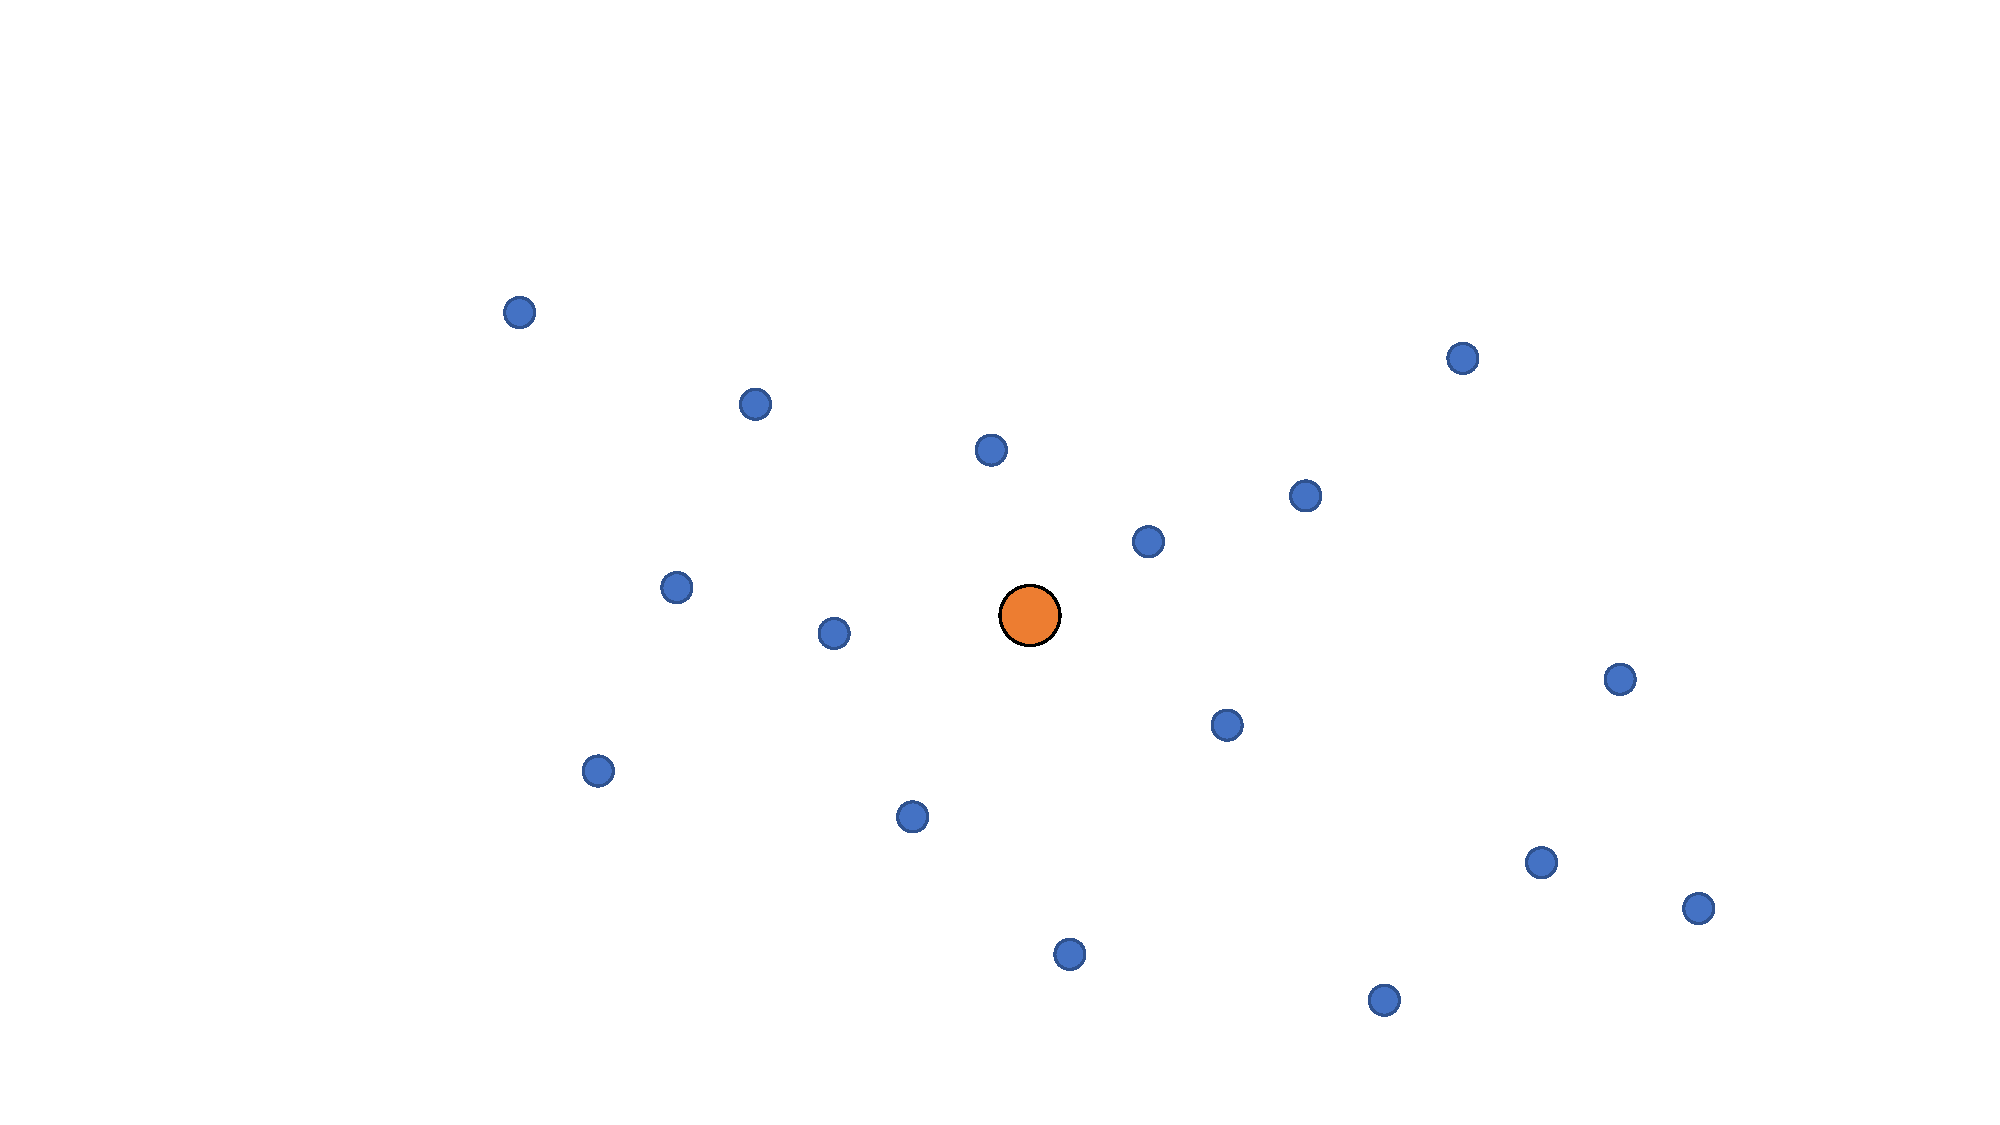
\includegraphics[width=0.75\linewidth]{../images/spatial_subd_find.pdf}
\end{center}





\newpage

\begin{center}
\begin{tabular}{|c|c|}
\hline
 & \\
\hspace{10pt}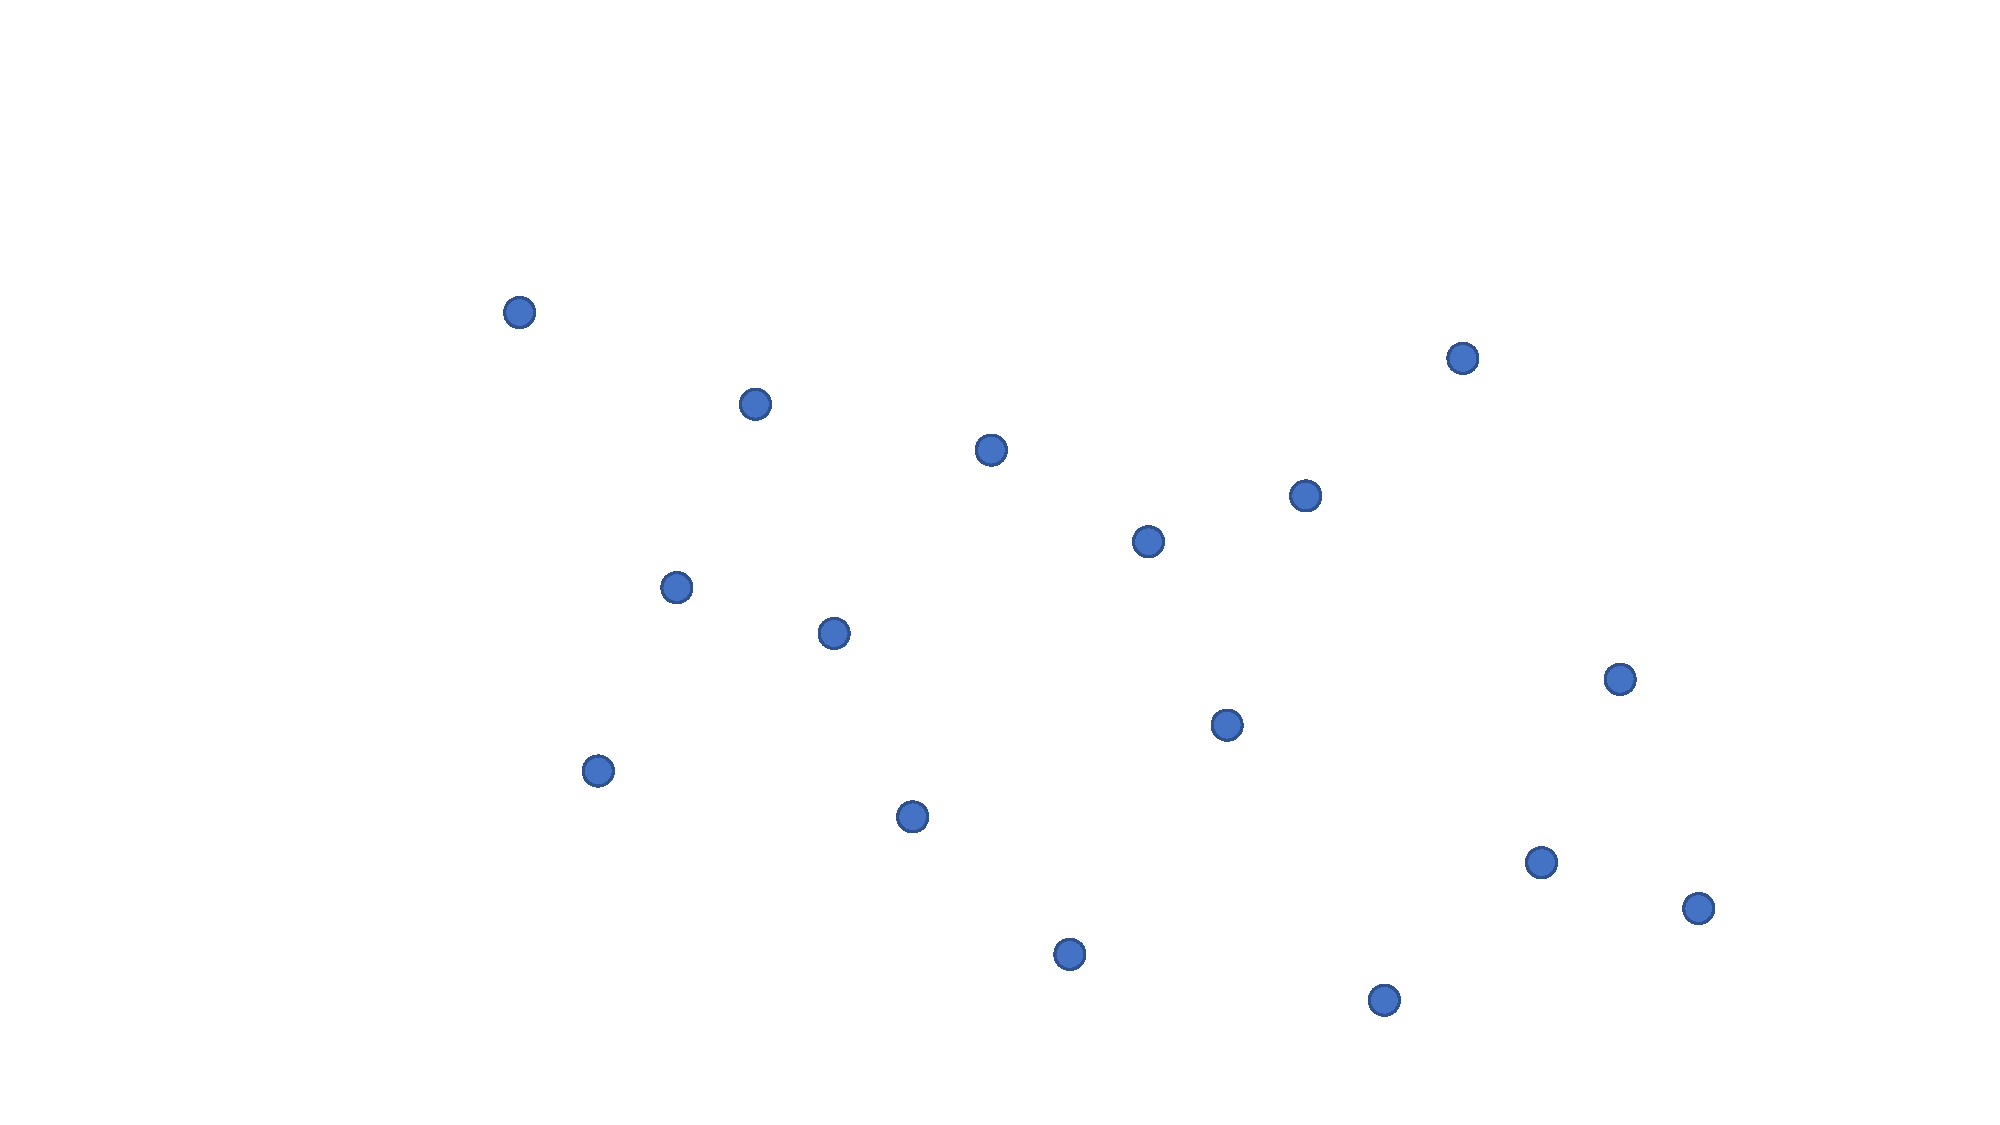
\includegraphics[width=7.5cm]{../images/spatial_subd.pdf}
\hspace{10pt} & \hspace{175pt} \\
 & \\
\hline
 & \\
\hspace{10pt}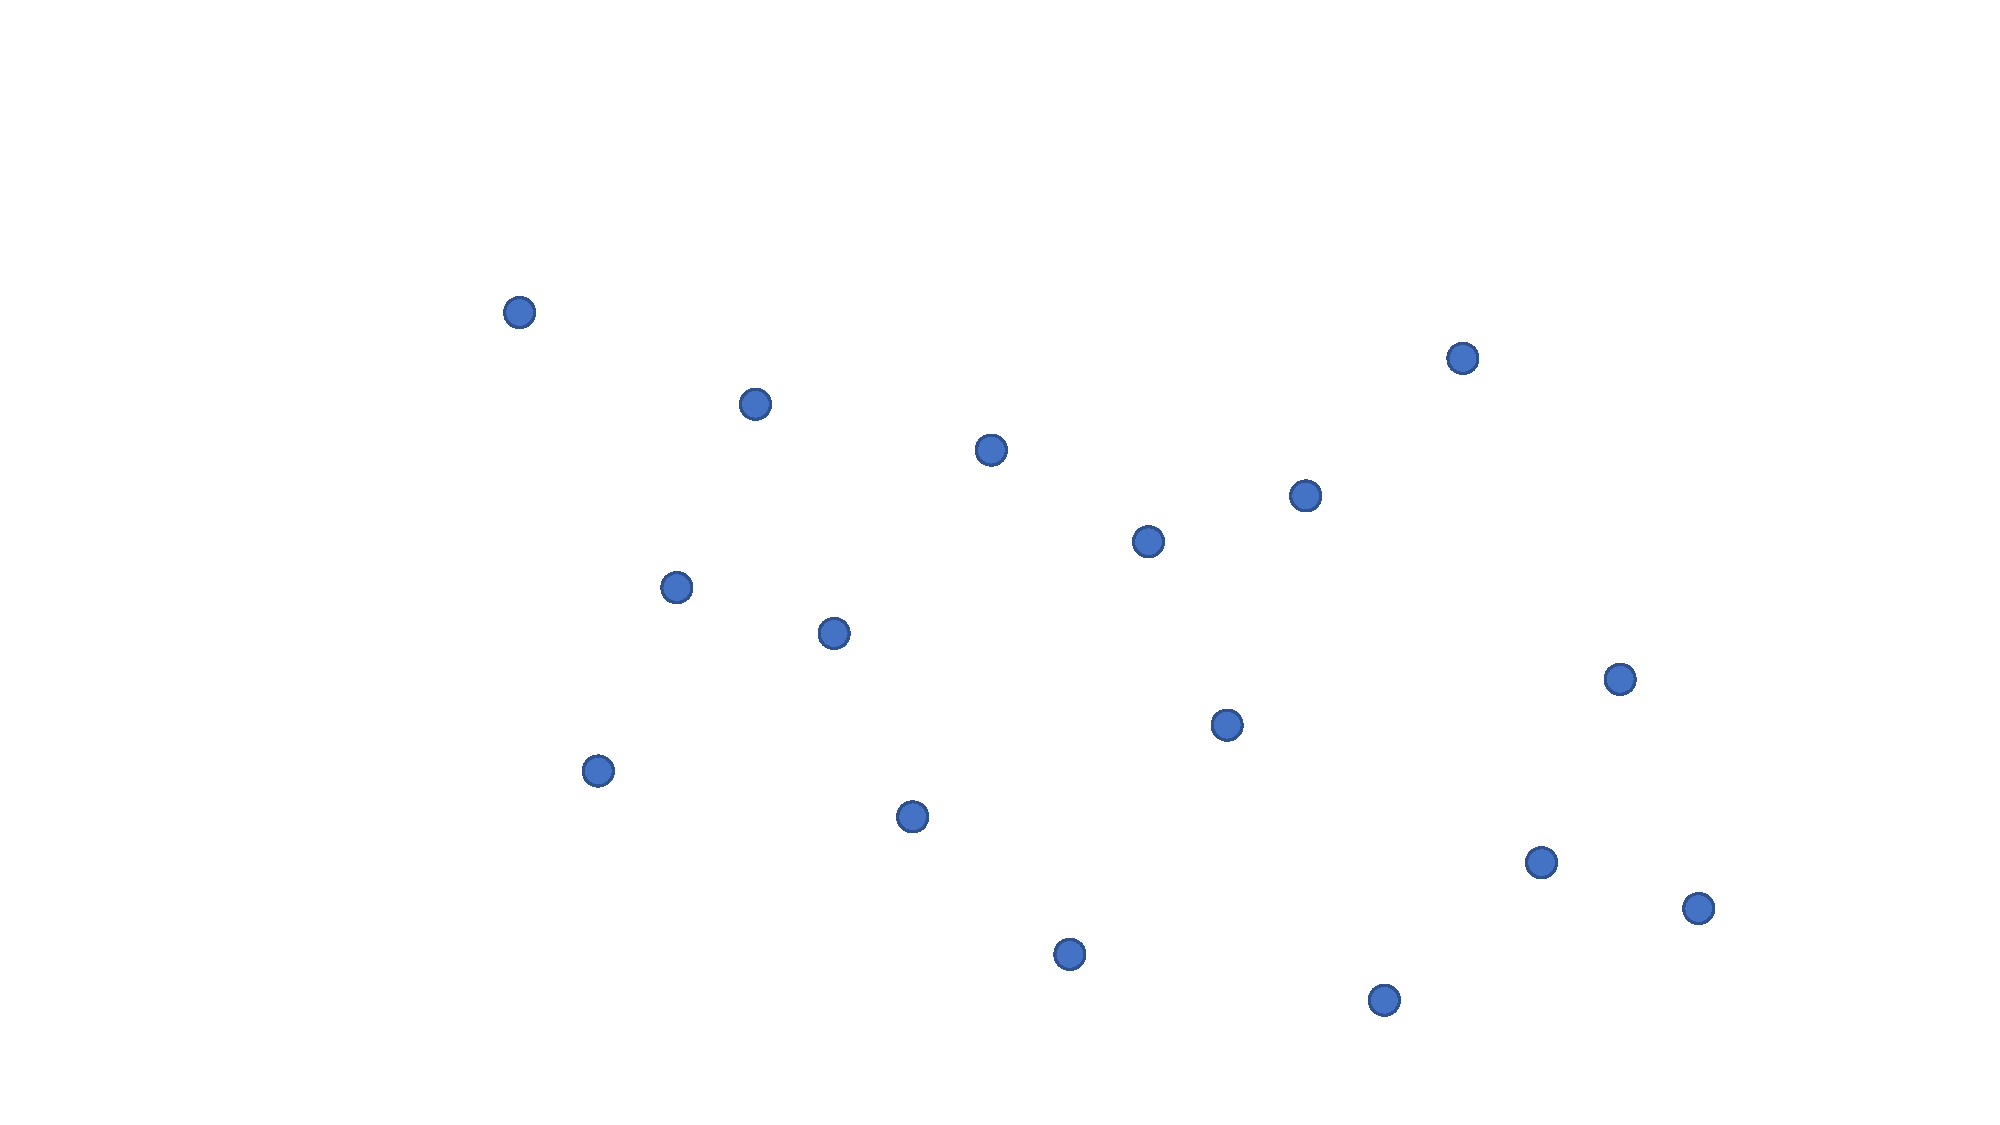
\includegraphics[width=7.5cm]{../images/spatial_subd.pdf}
\hspace{10pt} & \hspace{10pt} \\
 & \\
\hline
 & \\
\hspace{10pt}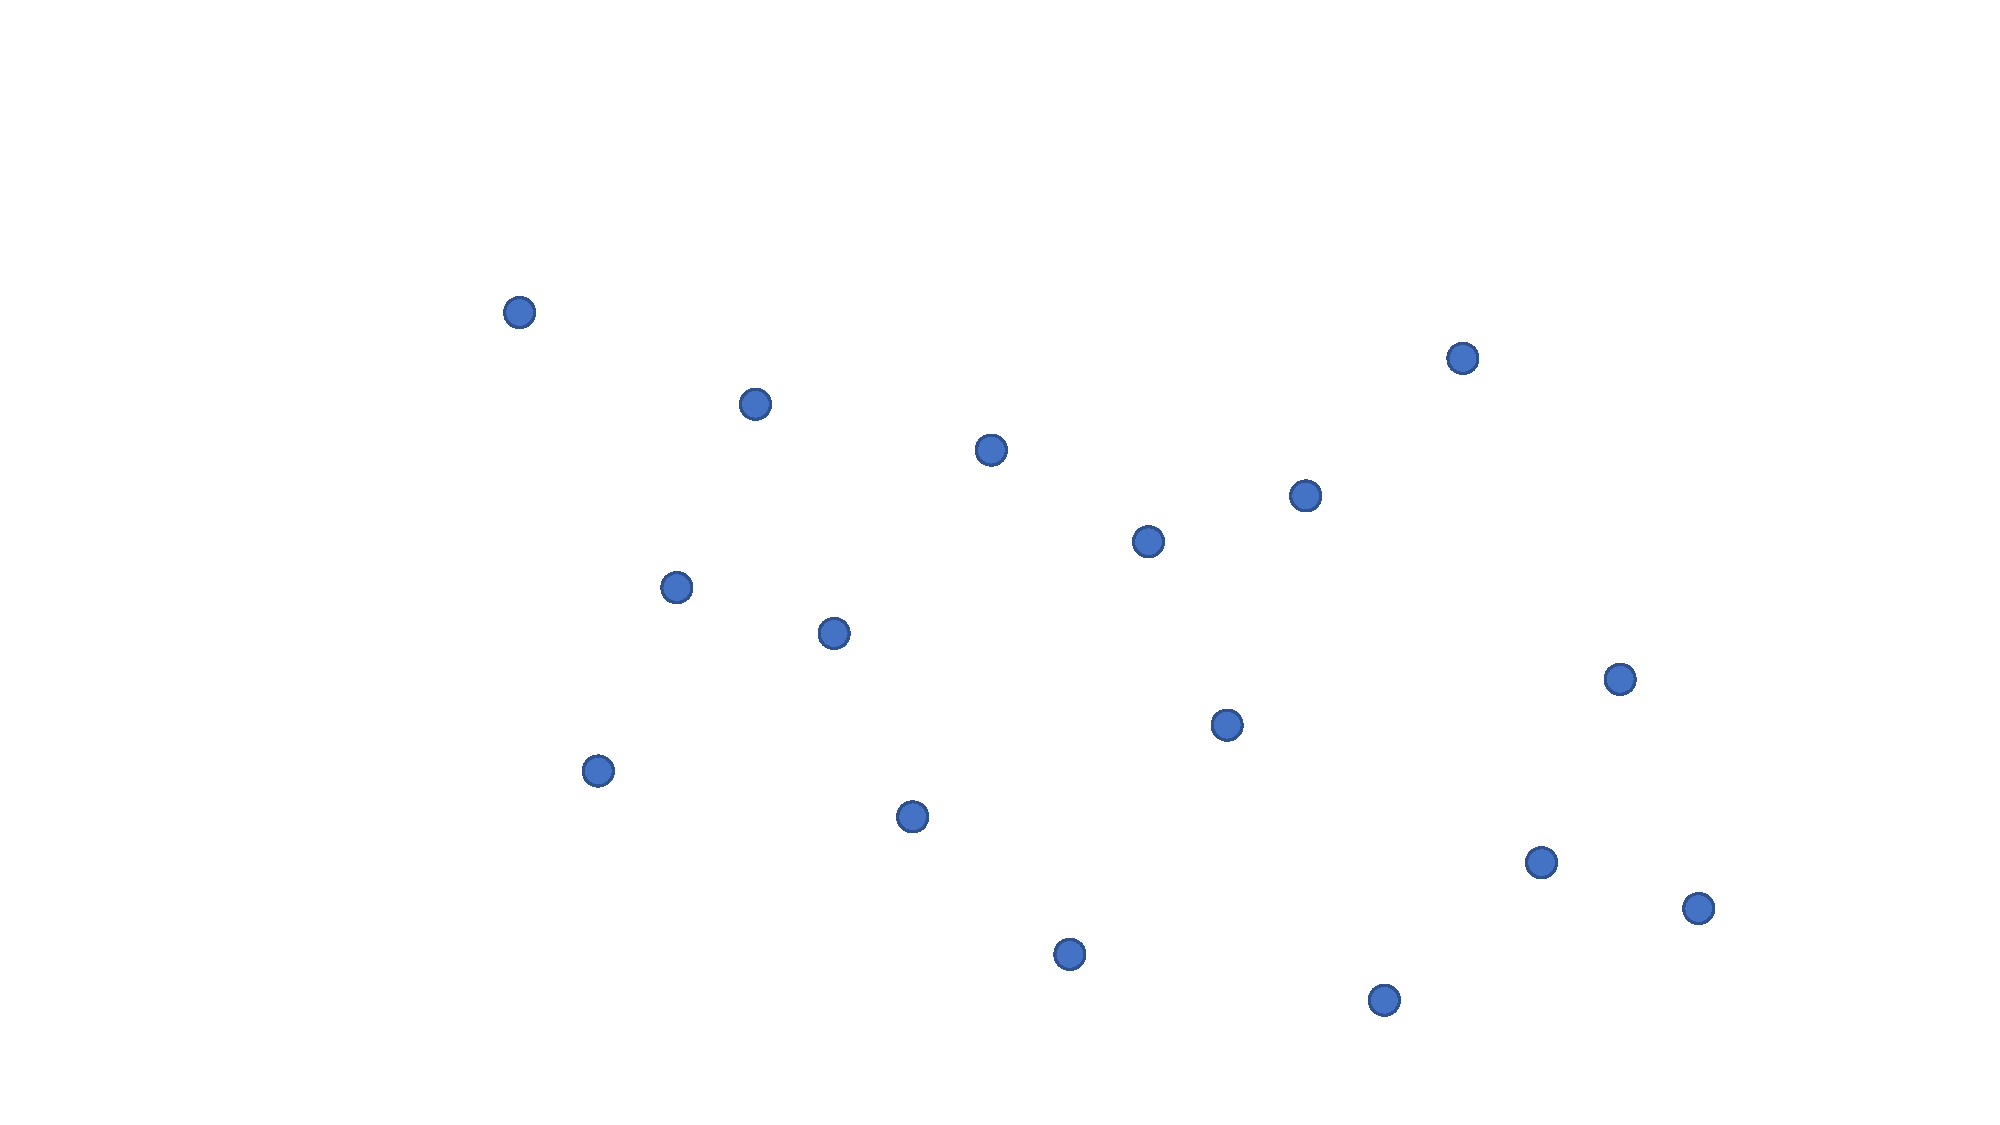
\includegraphics[width=7.5cm]{../images/spatial_subd.pdf}
\hspace{10pt} & \hspace{10pt} \\
 & \\
\hline
 & \\
\hspace{10pt}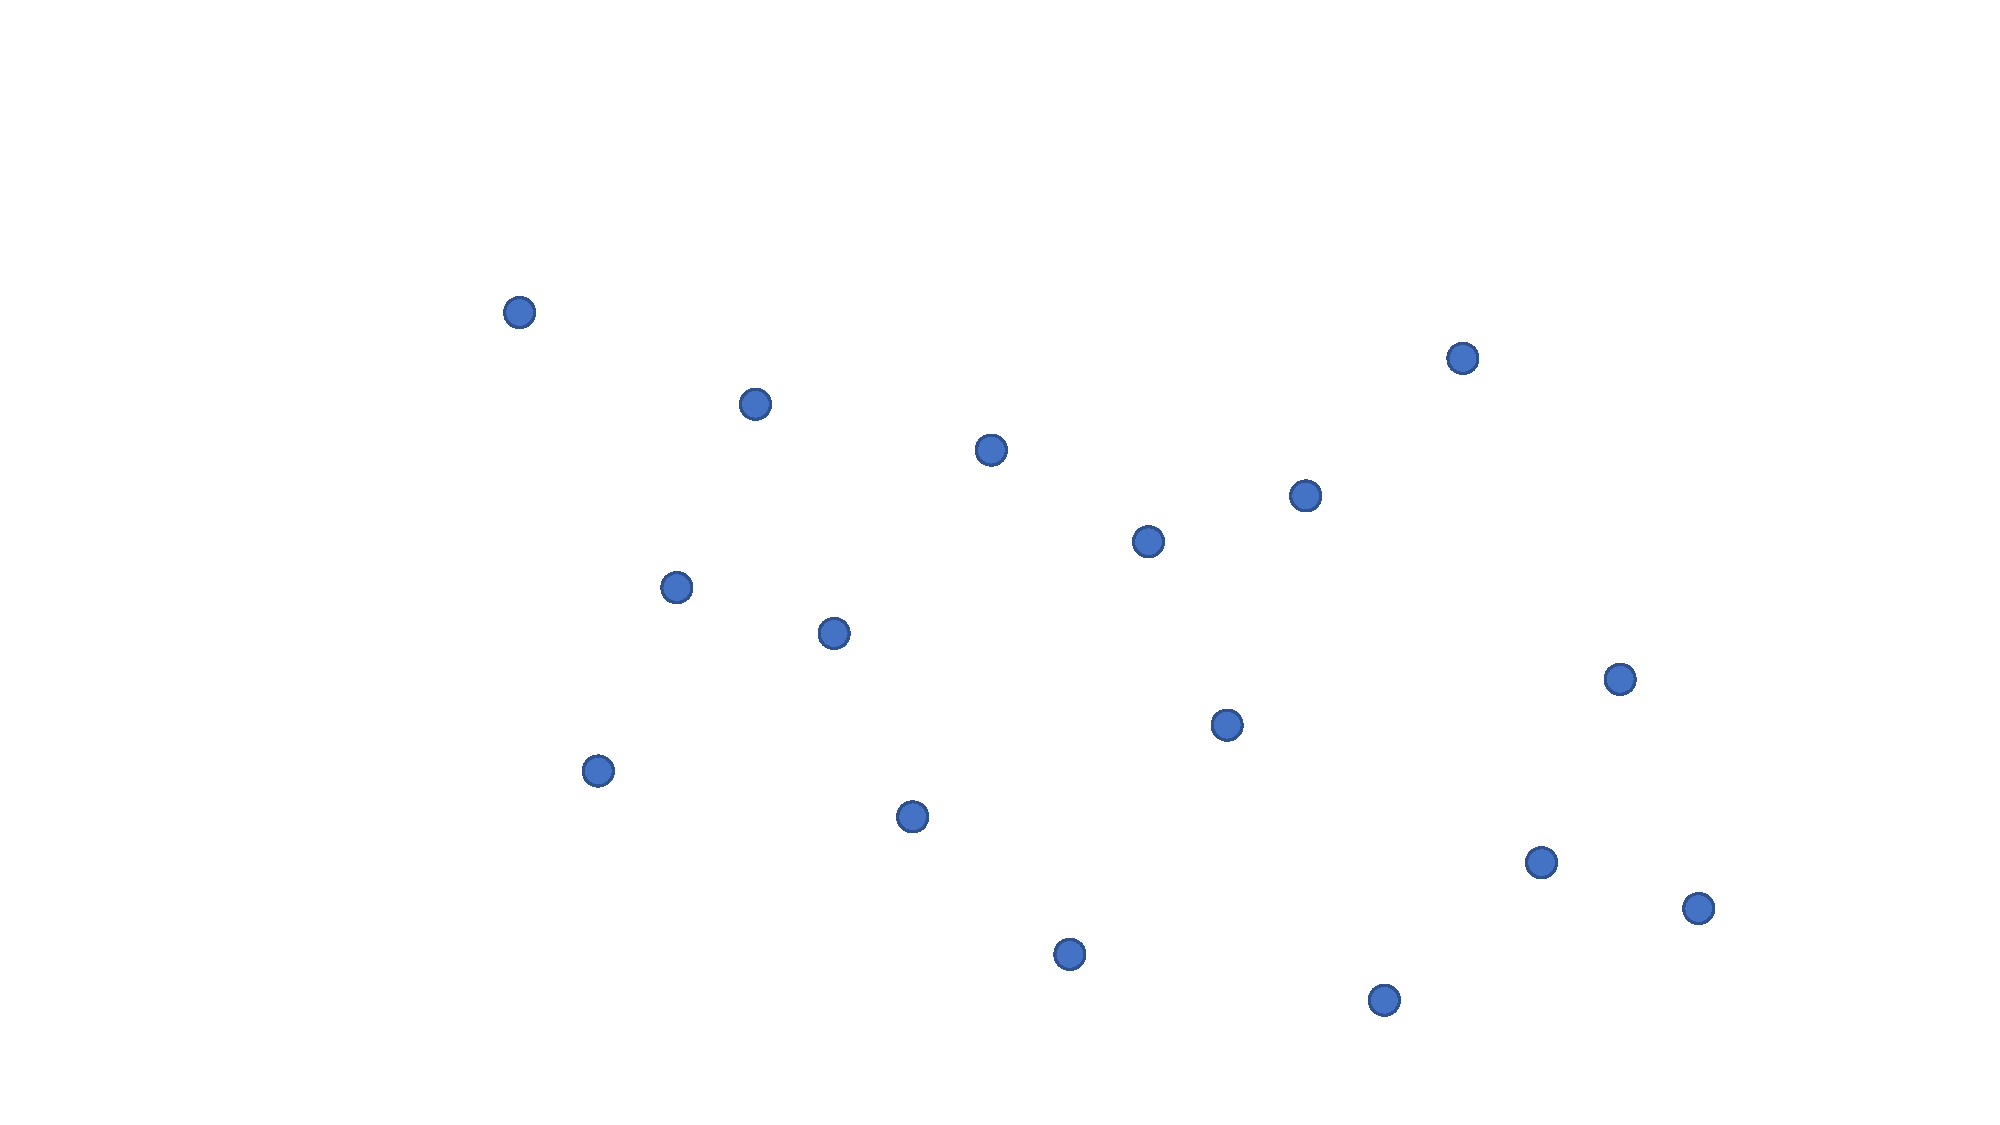
\includegraphics[width=7.5cm]{../images/spatial_subd.pdf}
\hspace{10pt} & \hspace{10pt} \\
 & \\
\hline
\end{tabular}
\end{center}



\newpage

\begin{center}
\begin{tabular}{|c|c|}
\hline
 & \\
\hspace{10pt}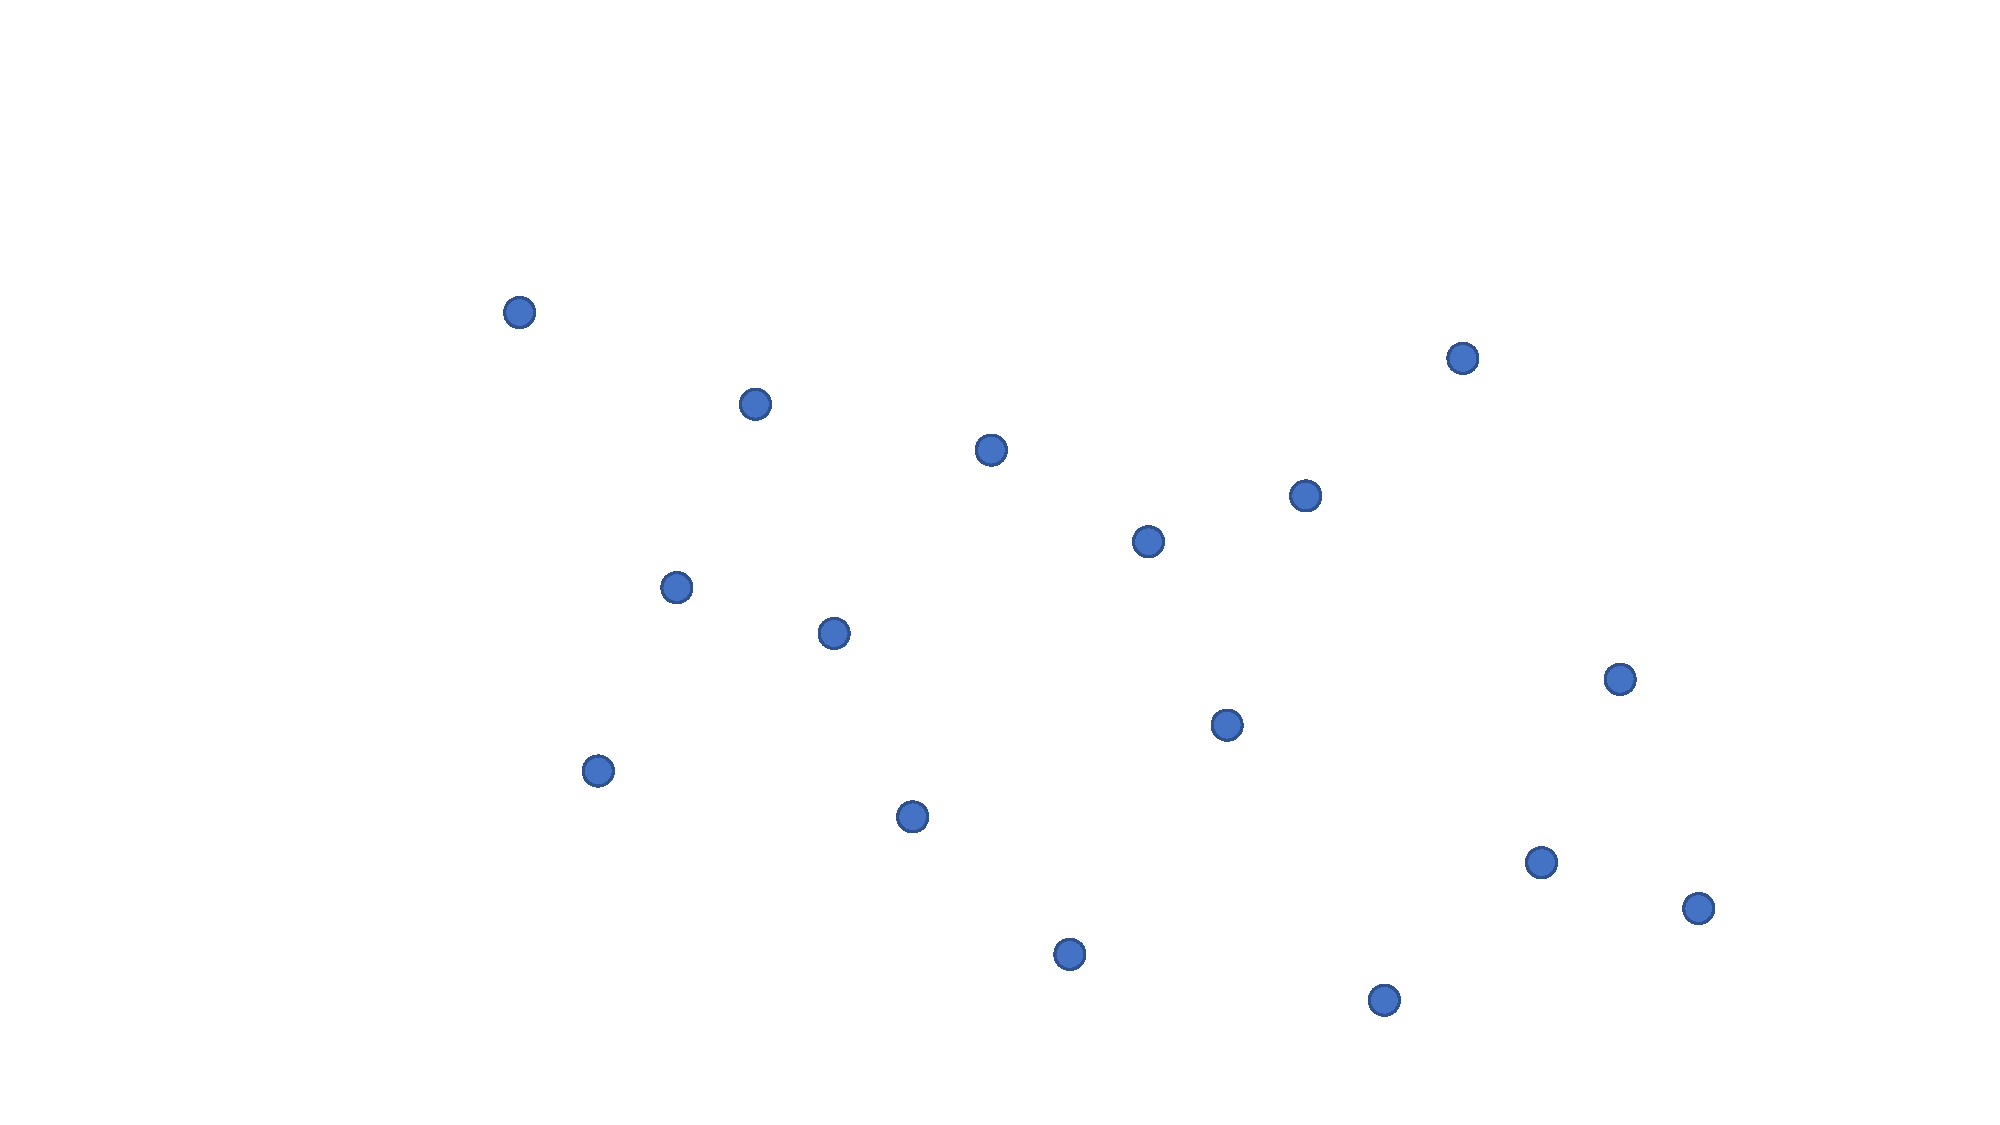
\includegraphics[width=7.5cm]{../images/spatial_subd.pdf}
\hspace{10pt} & \hspace{175pt} \\
 & \\
\hline
 & \\
\hspace{10pt}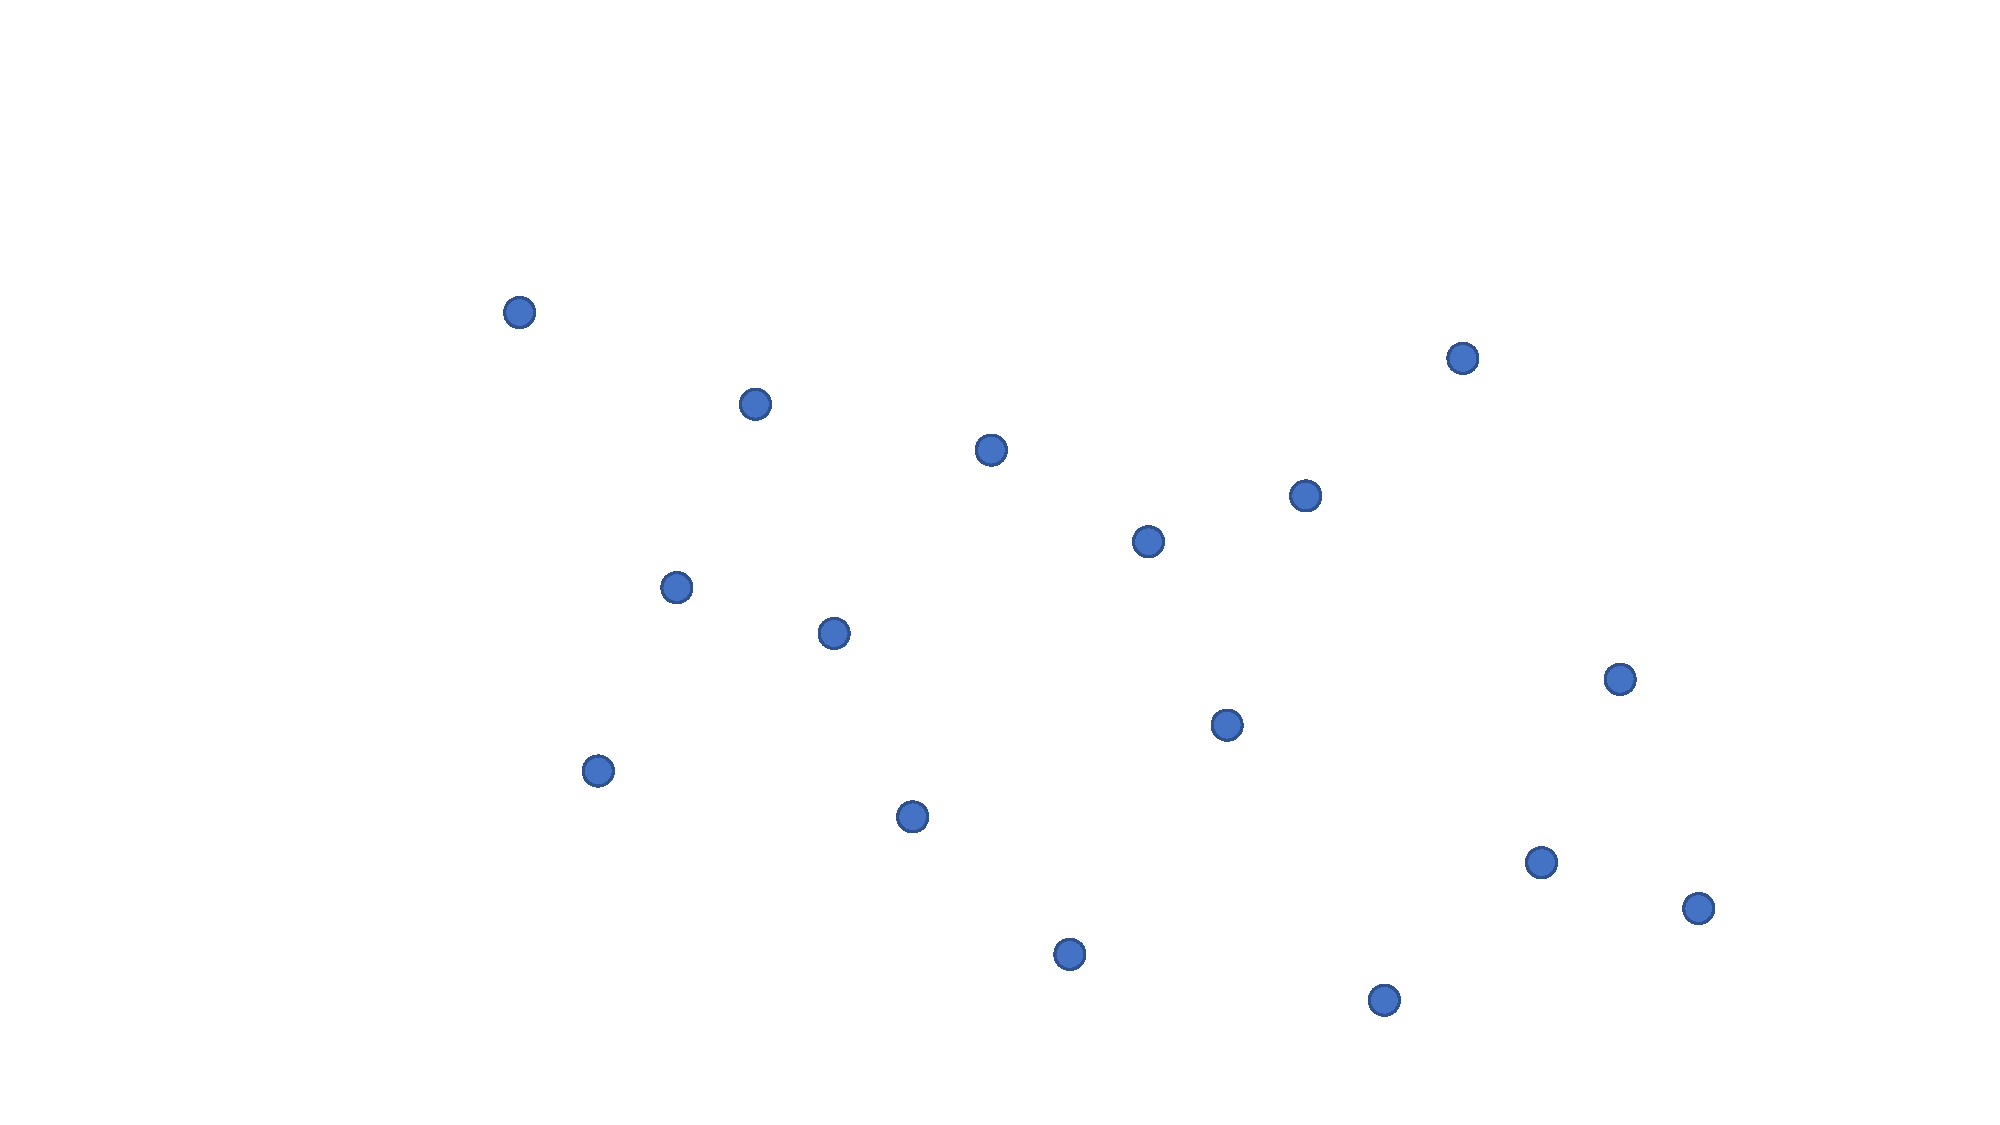
\includegraphics[width=7.5cm]{../images/spatial_subd.pdf}
\hspace{10pt} & \hspace{10pt} \\
 & \\
\hline
 & \\
\hspace{10pt}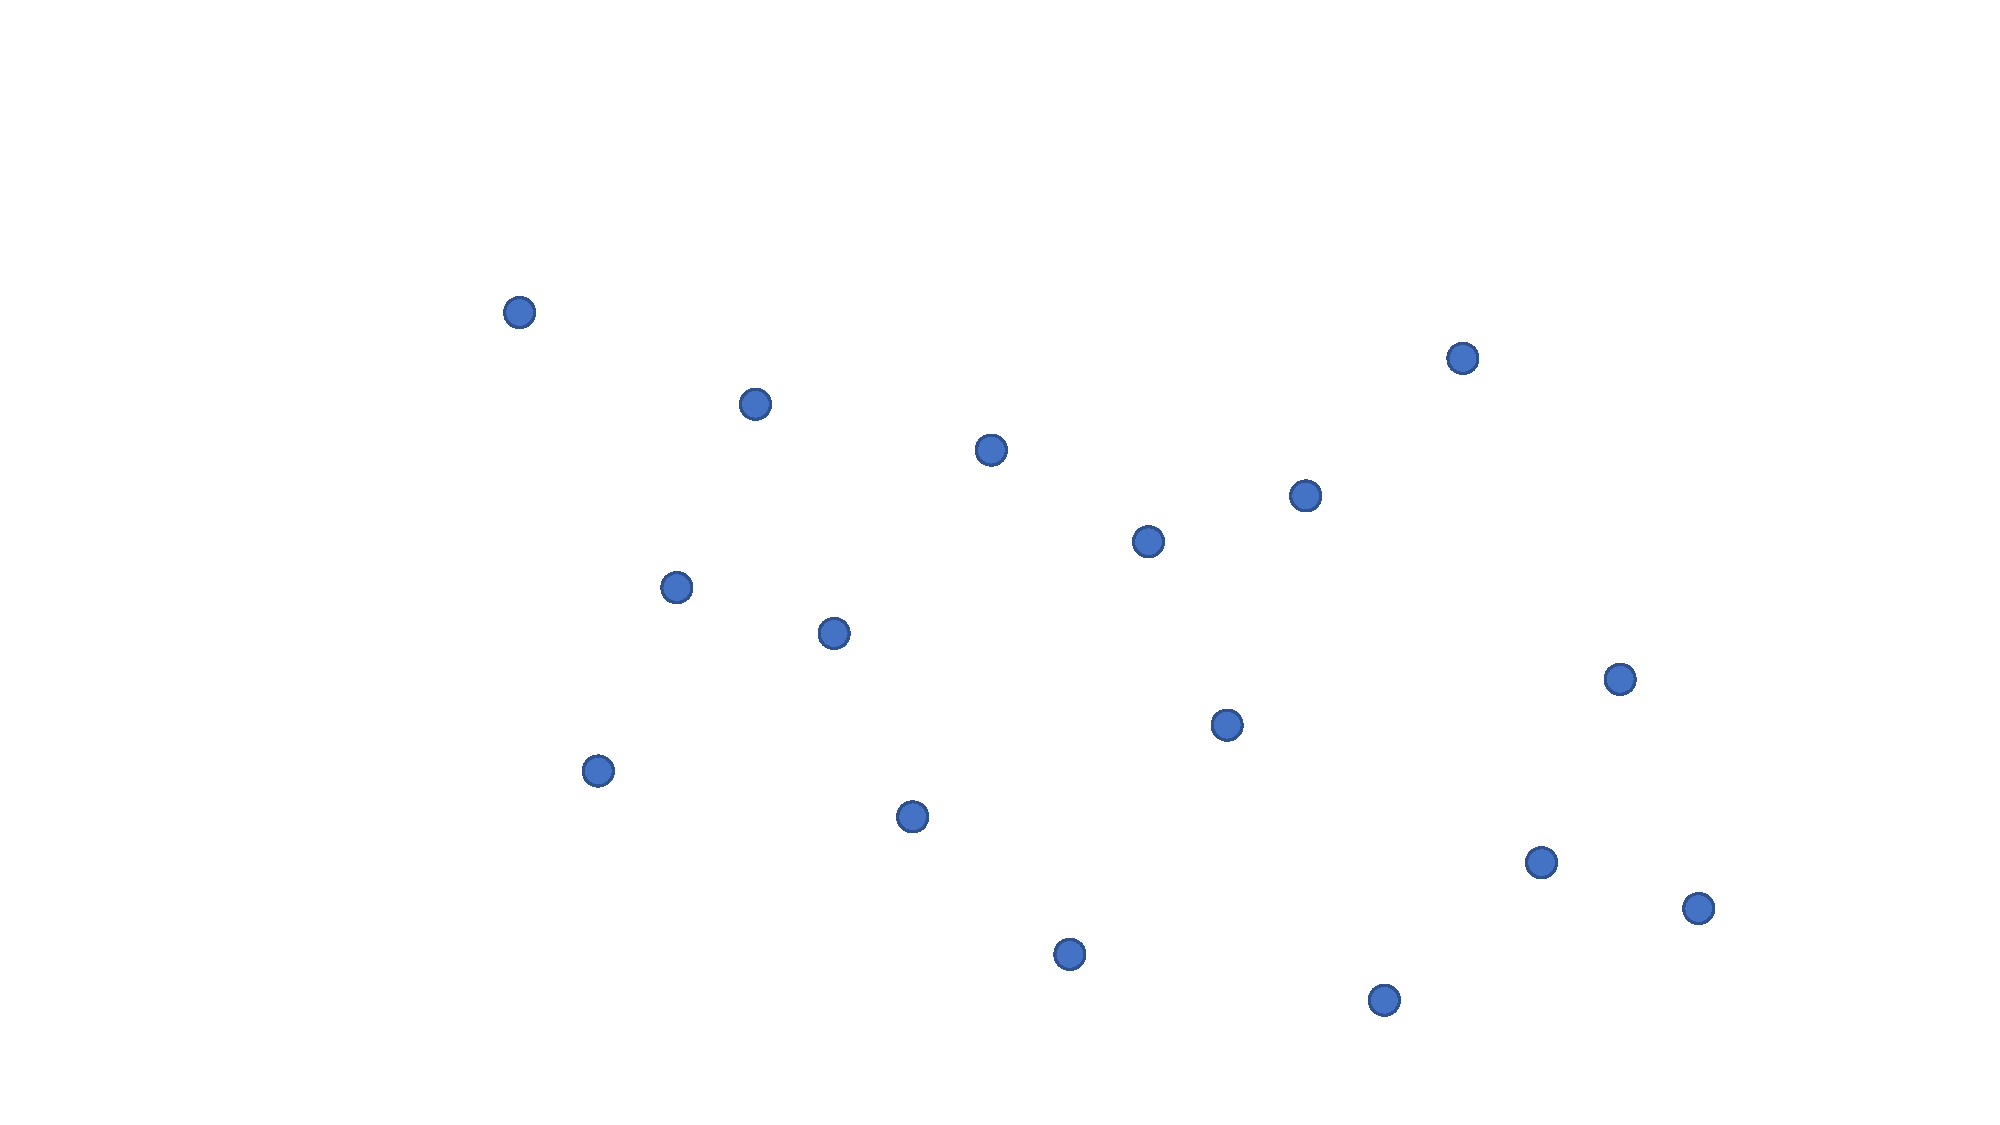
\includegraphics[width=7.5cm]{../images/spatial_subd.pdf}
\hspace{10pt} & \hspace{10pt} \\
 & \\
\hline
 & \\
\hspace{10pt}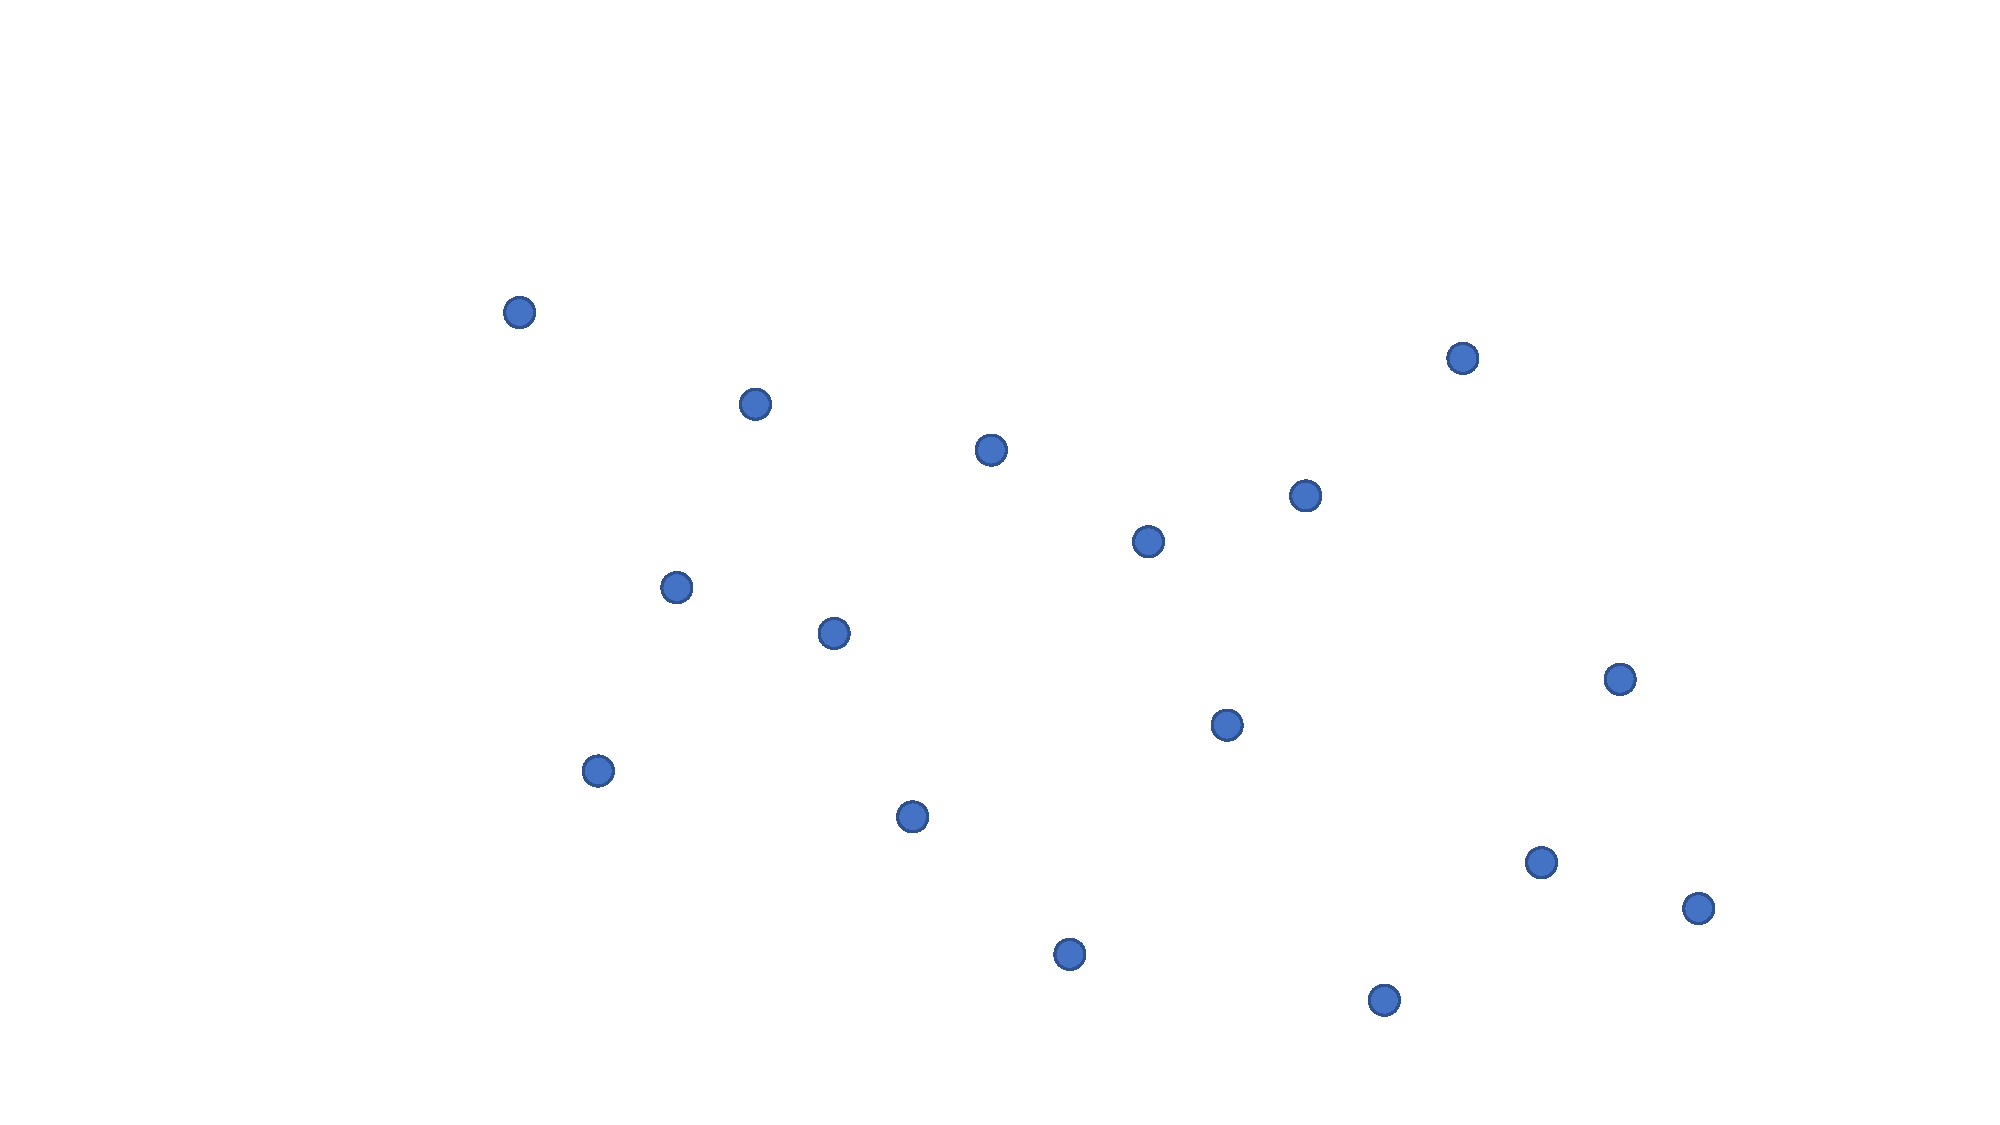
\includegraphics[width=7.5cm]{../images/spatial_subd.pdf}
\hspace{10pt} & \hspace{10pt} \\
 & \\
\hline
\end{tabular}
\end{center}



\newpage

\begin{center}
\begin{tabular}{|c|c|}
\hline
 & \\
\hspace{10pt}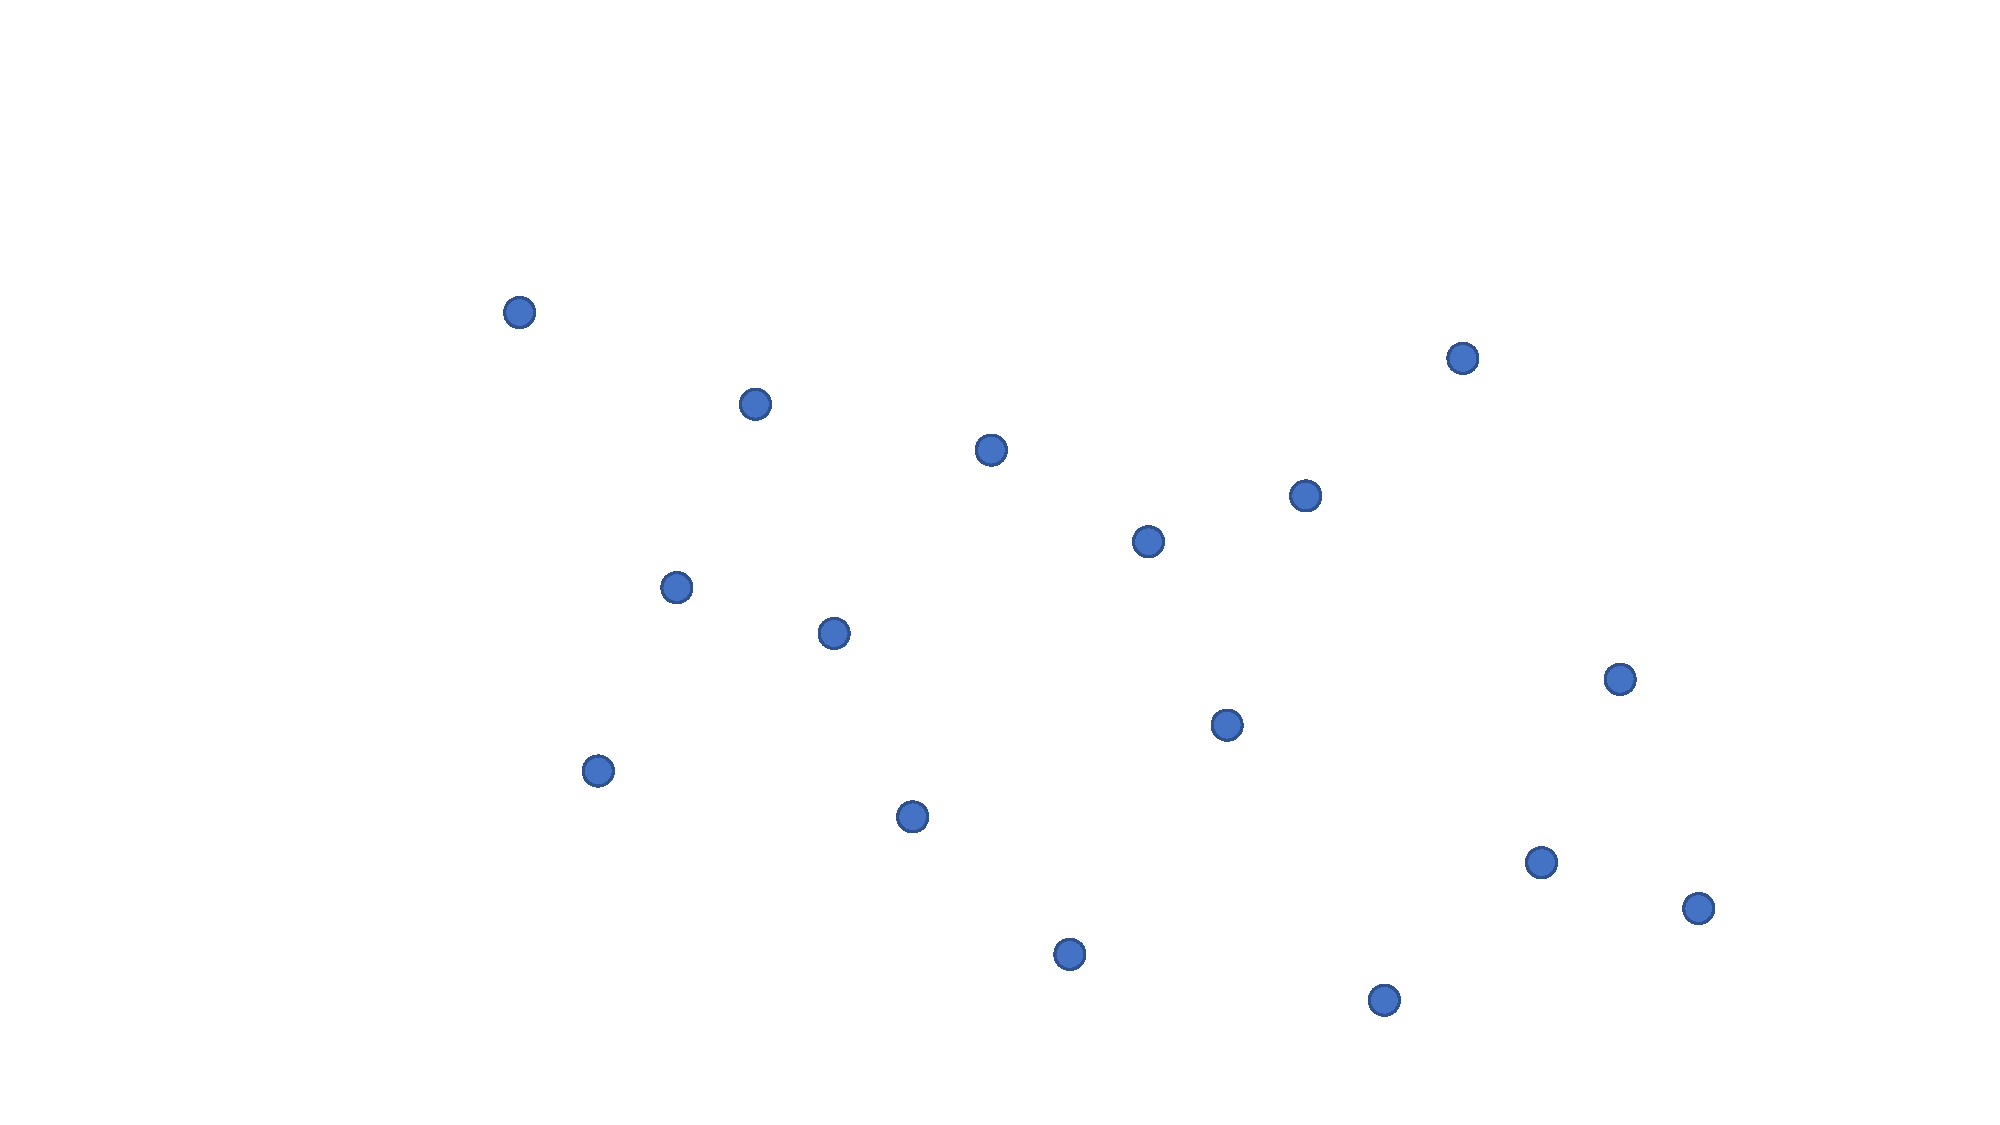
\includegraphics[width=7.5cm]{../images/spatial_subd.pdf}
\hspace{10pt} & \hspace{175pt} \\
 & \\
\hline
 & \\
\hspace{10pt}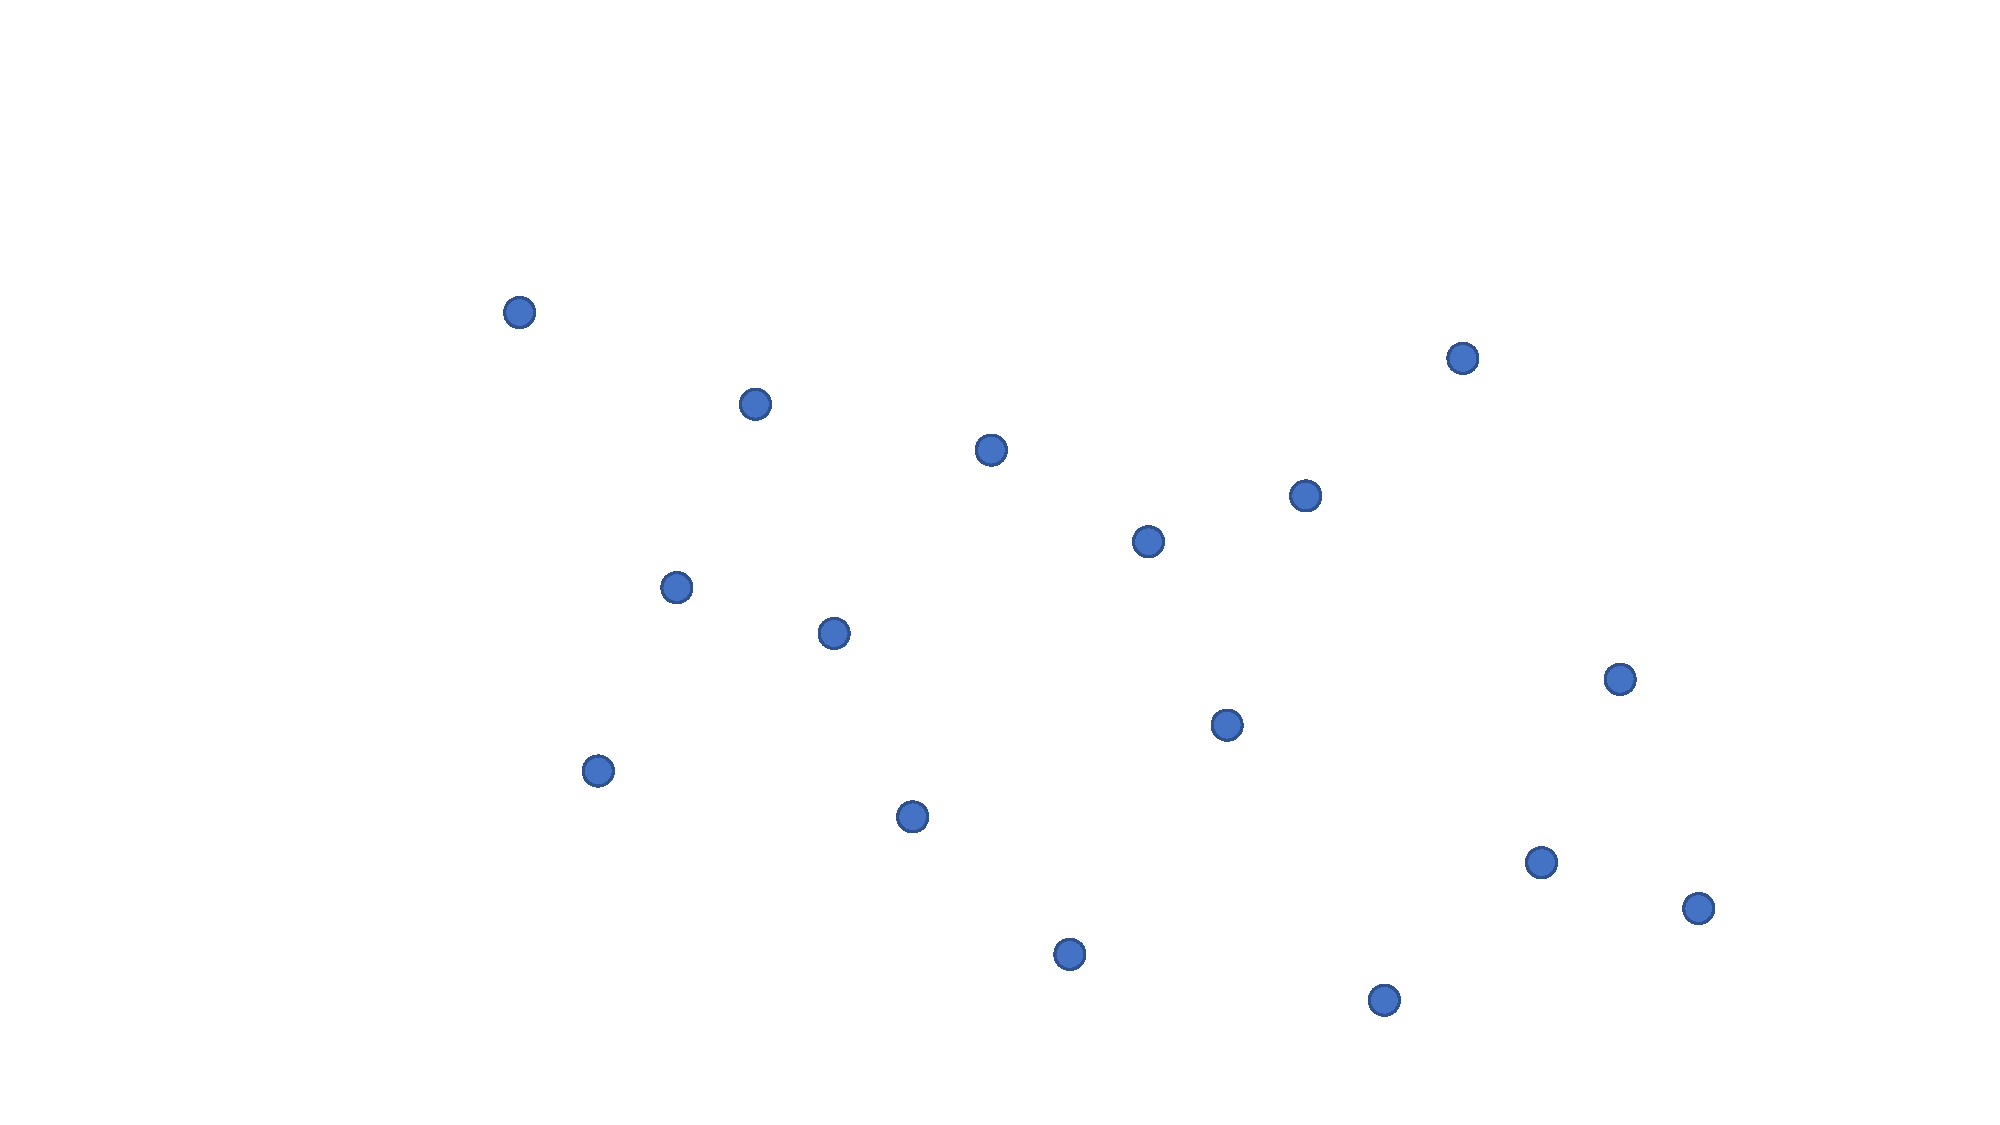
\includegraphics[width=7.5cm]{../images/spatial_subd.pdf}
\hspace{10pt} & \hspace{10pt} \\
 & \\
\hline
 & \\
\hspace{10pt}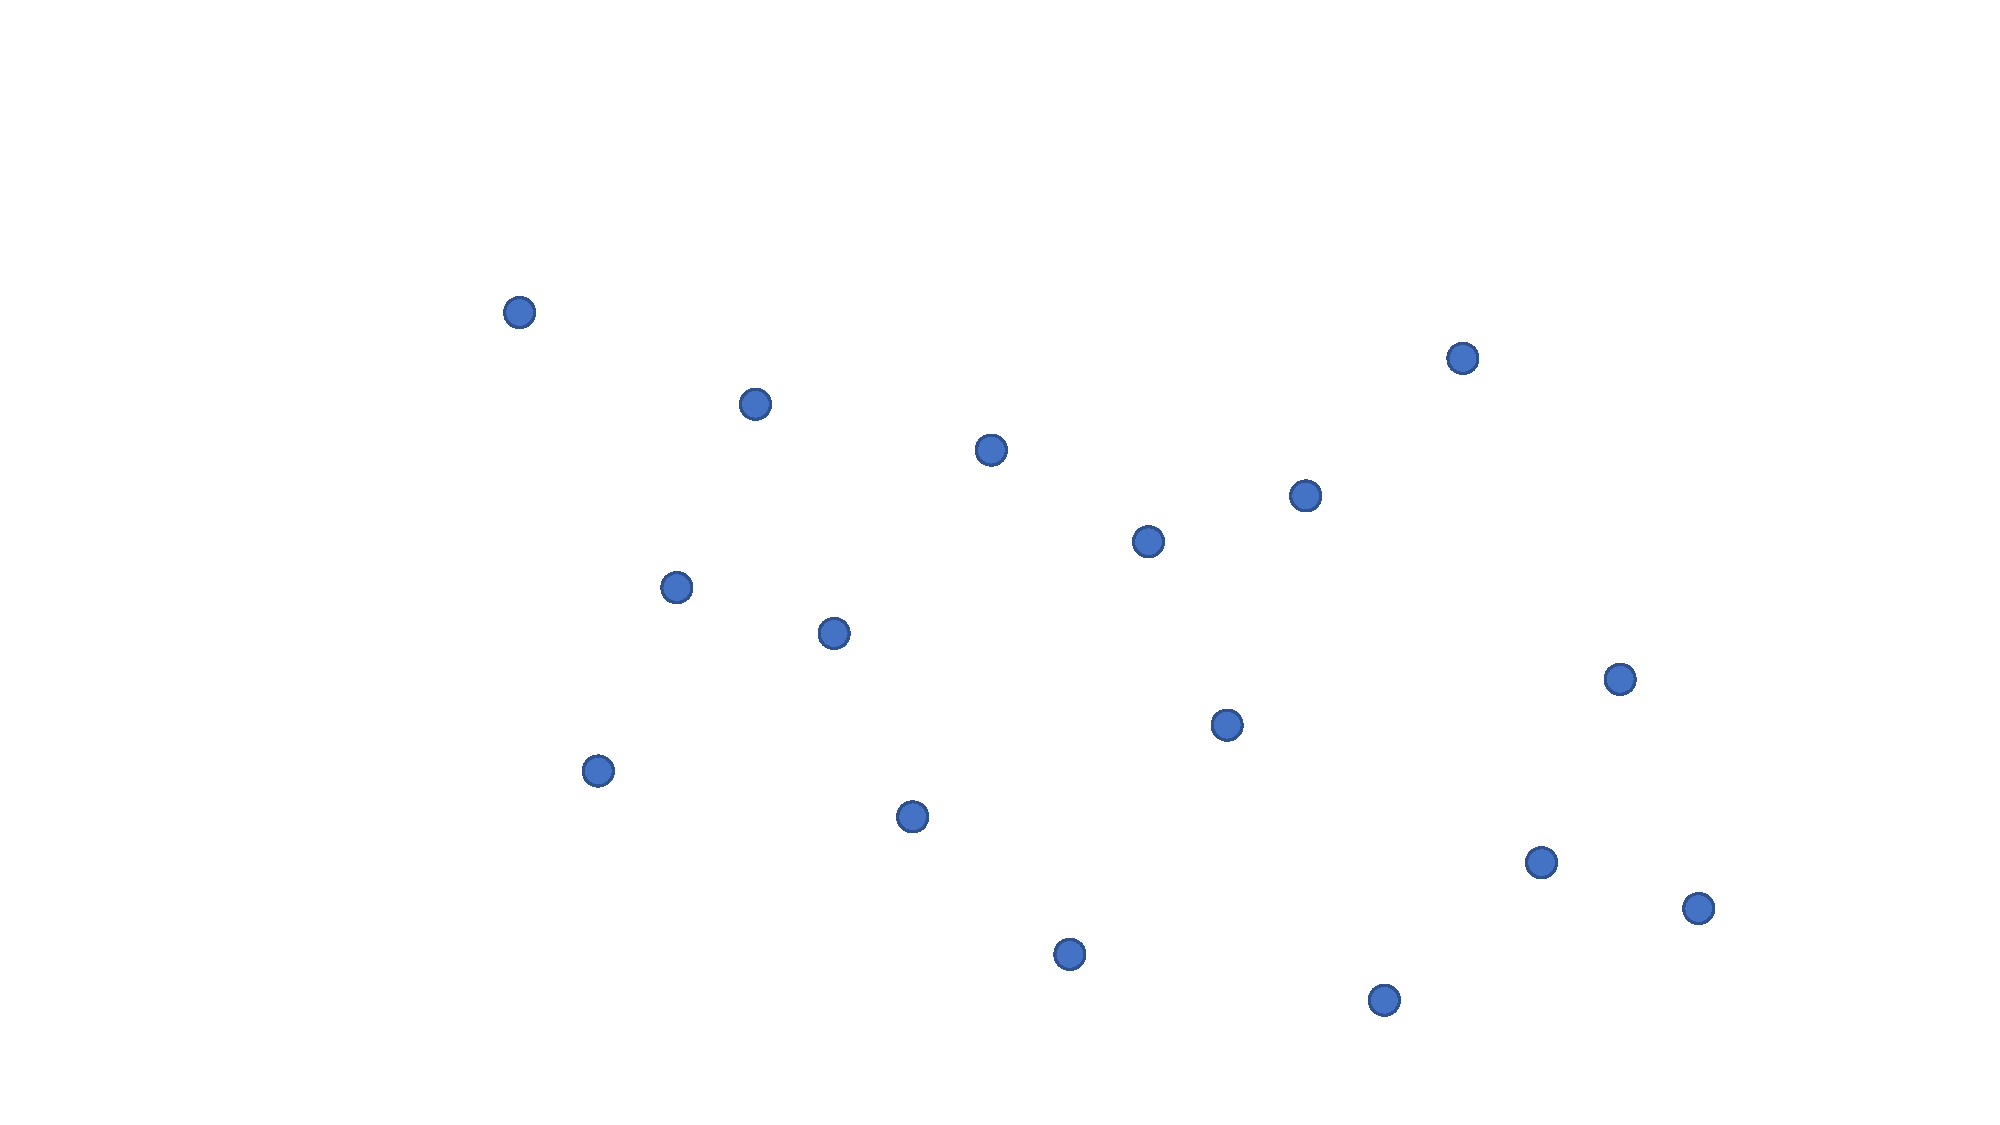
\includegraphics[width=7.5cm]{../images/spatial_subd.pdf}
\hspace{10pt} & \hspace{10pt} \\
 & \\
\hline
 & \\
\hspace{10pt}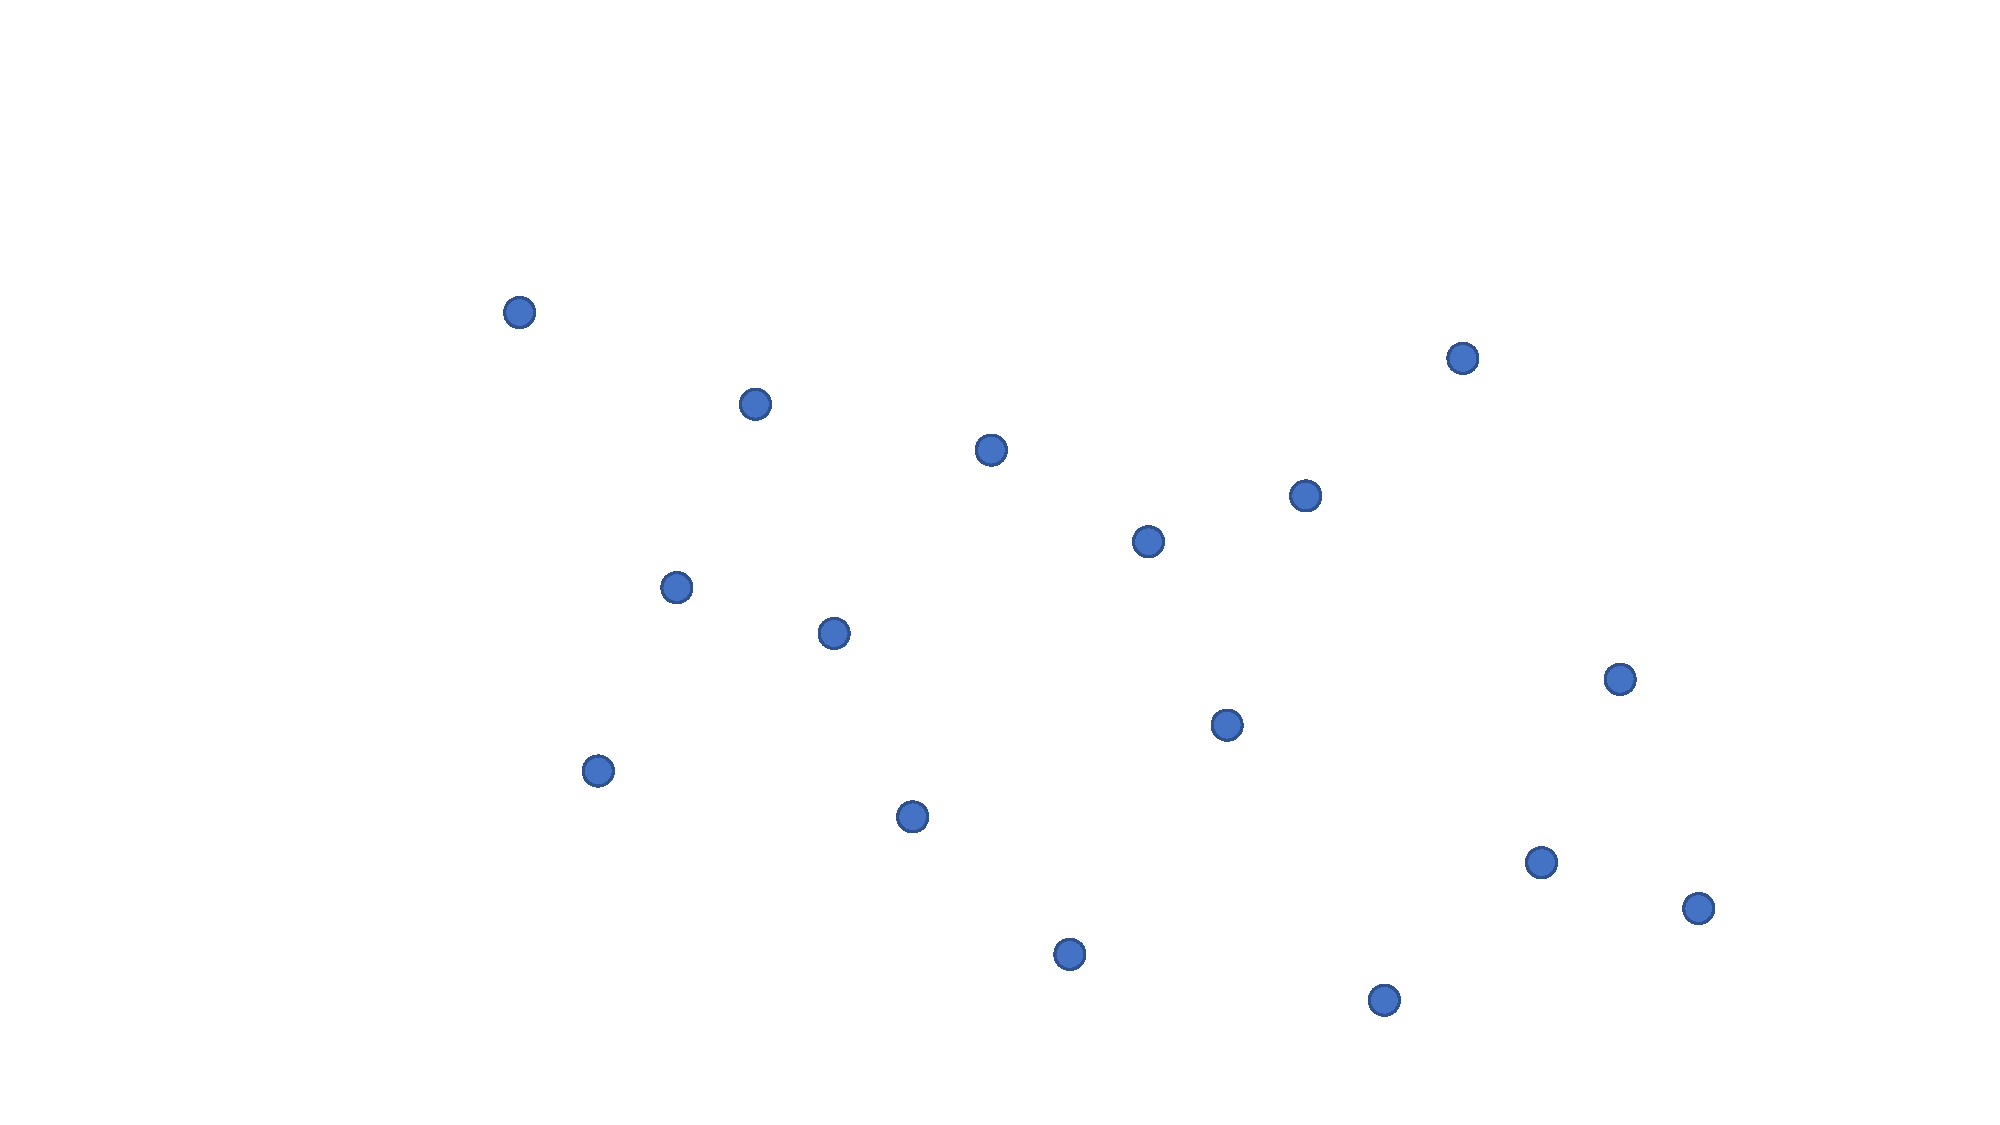
\includegraphics[width=7.5cm]{../images/spatial_subd.pdf}
\hspace{10pt} & \hspace{10pt} \\
 & \\
\hline
\end{tabular}
\end{center}


\end{document}



